\documentclass[aspectratio=169, 11pt]{beamer}

% --- Packages & Setup ---
\usepackage[utf8]{inputenc}
\usepackage[T1]{fontenc}
\usepackage{xcolor}
\usepackage{booktabs}
\usepackage{graphicx}
\usepackage{tikz}
\usetikzlibrary{calc,arrows.meta,positioning,shapes.geometric,backgrounds}

\graphicspath{{../}{./}{screenshots/}}

\IfFileExists{opensans.sty}{\usepackage[default,scale=0.95]{opensans}}{}

% --- Branding ---
\definecolor{amritaMaroon}{HTML}{A4123F}
\definecolor{lightMaroon}{HTML}{F7EAF0}
\definecolor{keyRed}{HTML}{D32F2F}
\definecolor{navy}{HTML}{1B2A4A}
\definecolor{phaseRed}{HTML}{C0392B}
\definecolor{diagBg}{HTML}{E4EEF3}
\definecolor{podFace}{HTML}{9FC7B8}
\definecolor{podTop}{HTML}{C9E4DA}
\definecolor{podSide}{HTML}{E0965C}
\definecolor{dbFill}{HTML}{FFFFFF}

\usetheme{Madrid}
\usecolortheme[named=amritaMaroon]{structure}
\setbeamertemplate{navigation symbols}{}
\setbeamertemplate{footline}[frame number]
\setbeamertemplate{itemize item}{\color{amritaMaroon}\small$\bullet$}
\renewcommand{\arraystretch}{1.15}

\newcommand{\hl}[1]{\textcolor{keyRed}{\textbf{#1}}}

\begin{document}

% ============================================================
% TITLE
% ============================================================
\begin{frame}
    \begin{tikzpicture}[remember picture,overlay]
        \node[fill=amritaMaroon, text=white, font=\bfseries\footnotesize, anchor=north east, rounded corners=2pt, inner sep=5pt]
        at ($(current page.north east) + (-0.2cm,-0.2cm)$)
        {Type 1: Research Project};
    \end{tikzpicture}

    \centering
    \IfFileExists{logo.png}{\includegraphics[width=2.8cm]{logo.png}\vspace{0.1cm}}{\vspace{0.4cm}}

    {\large \textbf{\textcolor{amritaMaroon}{PORYGON: A Statistical and Rule-Based Runtime Behavioural Framework for Containerized Workloads}}} \\
    \vspace{0.08cm}
    {\footnotesize \textbf{23CSE498 -- Project Phase 2 (Panel Review 1)} \quad | \quad \textbf{Team Number: 75}} \\
    \vspace{0.15cm}

    \begin{table}
        \centering
        \footnotesize
        \renewcommand{\arraystretch}{1.05}
        \begin{tabular}{|c|c|l|}
            \hline
            \textbf{S.No} & \textbf{Register Number} & \textbf{Student Name} \\
            \hline
            1 & CB.EN.U4CSE23504 & Ashin Varghese \\
            \hline
            2 & CB.EN.U4CSE23559 & Anurup Krishna \\
            \hline
            3 & CB.EN.U4CSE23628 & Krishnan S \\
            \hline
            4 & CB.EN.U4CSE23661 & Madhav Sreejith \\
            \hline
        \end{tabular}
    \end{table}
    \vspace{0.08cm}

    {\footnotesize Guide: \textbf{Dr Abirami K}, Assistant Professor, Department of CSE} \\
    \vspace{0.08cm}
    {\scriptsize \today}
\end{frame}

% ============================================================
% 0. BACKGROUND -- FOUNDATIONAL CONCEPTS
% ============================================================
\section{Background}
\begin{frame}{1. Background: Container, Image, Digest}
    \footnotesize
    \textbf{What is a \hl{container}?}
    \begin{itemize}\setlength\itemsep{1pt}
        \item An isolated process on a normal Linux host, fenced off by kernel \hl{namespaces} (its own view of processes, filesystem, network) and limited by \hl{cgroups} (its share of CPU and memory).
        \item It \hl{shares the host kernel}, so it is far lighter than a virtual machine, which carries a whole operating system of its own.
    \end{itemize}
    \vspace{0.12cm}
    \textbf{What is a \hl{Docker image}?}
    \begin{itemize}\setlength\itemsep{1pt}
        \item A \hl{read-only template} a container is started from: stacked filesystem \hl{layers} plus a configuration document (entrypoint, environment, user).
        \item An image never changes once built. A container is one \hl{running instance} of it.
    \end{itemize}
    \vspace{0.12cm}
    \textbf{What is an image \hl{digest}?}
    \begin{itemize}\setlength\itemsep{1pt}
        \item A \hl{SHA-256 hash of the image manifest}, written \texttt{sha256:9b7f...}, that names the image by its exact content. Same bytes, same digest, always.
        \item A tag such as \texttt{nginx:latest} is only a \hl{movable pointer}; it can be repointed to different content tomorrow. The digest is the \hl{immutable identity}, which is why Porygon binds every baseline to it.
    \end{itemize}
    \vspace{0.1cm}
    \scriptsize Terminology follows the OCI Image Format Specification and the OCI Runtime Specification \cite{ociimage}.
\end{frame}

% ============================================================
% 1b. BACKGROUND -- VISUAL: IMAGE, CONTAINER, DIGEST
% ============================================================
\begin{frame}{2. Background: From Image to Running Container}
    \centering
    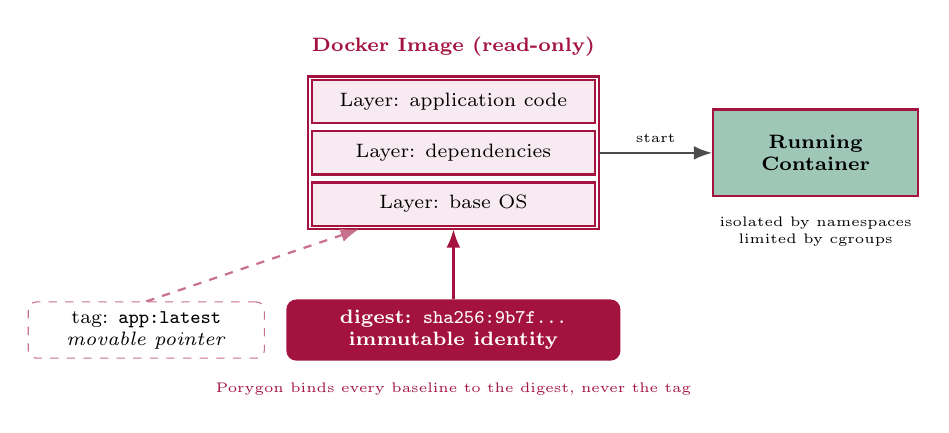
\begin{tikzpicture}[
        font=\scriptsize,
        layer/.style={draw=amritaMaroon, thick, fill=lightMaroon, minimum width=3.6cm, minimum height=0.55cm, align=center},
        tagbox/.style={draw=amritaMaroon!60, dashed, rounded corners=3pt, fill=white, minimum width=3.0cm, minimum height=0.6cm, align=center, font=\scriptsize},
        digestbox/.style={draw=amritaMaroon, very thick, rounded corners=3pt, fill=amritaMaroon, text=white, minimum width=4.2cm, minimum height=0.7cm, align=center, font=\bfseries\scriptsize},
        podb/.style={draw=amritaMaroon, thick, fill=podFace, minimum width=2.6cm, minimum height=1.1cm, align=center, font=\bfseries\scriptsize},
        arr/.style={-Latex, thick, draw=black!70}
    ]
        % --- stacked image layers ---
        \node[layer] (l1) at (0,0) {Layer: base OS};
        \node[layer] (l2) at (0,0.65) {Layer: dependencies};
        \node[layer] (l3) at (0,1.3) {Layer: application code};
        \draw[draw=amritaMaroon, thick] (-1.85,-0.32) rectangle (1.85,1.62);
        \node[font=\bfseries\scriptsize, color=amritaMaroon] at (0,2.0) {Docker Image (read-only)};

        % --- tag vs digest, both pointing at the same image ---
        \node[tagbox] (tag) at (-3.9,-1.6) {tag: \texttt{app:latest}\\\scriptsize\emph{movable pointer}};
        \node[digestbox] (digest) at (0,-1.6) {digest: \texttt{sha256:9b7f...}\\\scriptsize immutable identity};
        \draw[arr, dashed, amritaMaroon!60] (tag.north) -- (-1.2,-0.32);
        \draw[arr, amritaMaroon] (digest.north) -- (0,-0.32);

        % --- container instance spawned from the image ---
        \node[podb] (container) at (4.6,0.65) {Running\\Container};
        \draw[arr] (1.85,0.65) -- (container.west) node[midway, above, font=\tiny] {start};
        \node[font=\tiny, align=center] at (4.6,-0.35) {isolated by namespaces\\limited by cgroups};

        \node[font=\tiny, color=amritaMaroon] at (0,-2.35) {Porygon binds every baseline to the digest, never the tag};
    \end{tikzpicture}
\end{frame}

% ============================================================
% 1. INTRODUCTION
% ============================================================
\section{Introduction}
\begin{frame}{3. Introduction}
    \begin{columns}[T]
        \column{0.53\textwidth}
        \footnotesize
        \textbf{Background}
        \begin{itemize}\setlength{\itemsep}{5pt}
            \item Containers continuously emit process-execution and lifecycle events.
            \item Porygon learns each image's expected runtime behaviour.
            \item New activity is compared to that baseline using Jensen--Shannon distance.
            \item Deterministic rules attach explainable evidence to any deviation.
        \end{itemize}
        \vspace{0.15cm}
        \textbf{Objective}
        \begin{block}{}
            \scriptsize Build an image-specific runtime framework that measures behavioural deviation and produces explainable findings.
        \end{block}

        \column{0.44\textwidth}
        \centering
        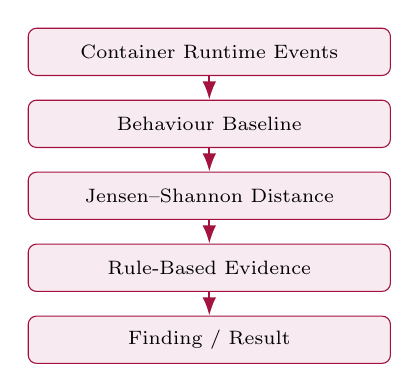
\begin{tikzpicture}[node distance=0.3cm,
            box/.style={draw=amritaMaroon,rounded corners=3pt,fill=lightMaroon,
                        minimum width=4.6cm,minimum height=0.6cm,align=center,font=\scriptsize},
            arrow/.style={-Latex,thick,draw=amritaMaroon}]
            \node[box] (events) {Container Runtime Events};
            \node[box,below=of events] (baseline) {Behaviour Baseline};
            \node[box,below=of baseline] (score) {Jensen--Shannon Distance};
            \node[box,below=of score] (rules) {Rule-Based Evidence};
            \node[box,below=of rules] (finding) {Finding / Result};
            \draw[arrow] (events)--(baseline);
            \draw[arrow] (baseline)--(score);
            \draw[arrow] (score)--(rules);
            \draw[arrow] (rules)--(finding);
        \end{tikzpicture}
    \end{columns}
\end{frame}

% ============================================================
% 2. PROBLEM STATEMENT
% ============================================================
\section{Problem Statement}
\begin{frame}{4. Problem Statement}
    \vspace{0.25cm}
    \begin{center}
    \fboxsep=12pt\fboxrule=1.6pt
    \fcolorbox{amritaMaroon}{lightMaroon}{%
    \begin{minipage}{0.86\textwidth}
        \centering\Large
        A \hl{shared baseline} across different images causes \hl{false alarms}: Porygon scores each image against \hl{its own measured baseline}.
    \end{minipage}%
    }
    \end{center}

    \vspace{0.5cm}
    \textbf{\footnotesize Project Focus}
    \begin{columns}[T]
        \column{0.25\textwidth}\centering\footnotesize
        \fcolorbox{amritaMaroon}{lightMaroon}{\parbox[c][0.85cm][c]{0.9\linewidth}{\centering Baseline\\scoping}}
        \column{0.25\textwidth}\centering\footnotesize
        \fcolorbox{amritaMaroon}{lightMaroon}{\parbox[c][0.85cm][c]{0.9\linewidth}{\centering JSD\\scoring}}
        \column{0.25\textwidth}\centering\footnotesize
        \fcolorbox{amritaMaroon}{lightMaroon}{\parbox[c][0.85cm][c]{0.9\linewidth}{\centering Rule-based\\evidence}}
        \column{0.25\textwidth}\centering\footnotesize
        \fcolorbox{amritaMaroon}{lightMaroon}{\parbox[c][0.85cm][c]{0.9\linewidth}{\centering Controlled\\evaluation}}
    \end{columns}
\end{frame}

% ============================================================
% 3. LITERATURE REVIEW -- AS A DIAGRAM
% ============================================================
\section{Literature Review}
\begin{frame}{5. Literature Review}
    \centering
    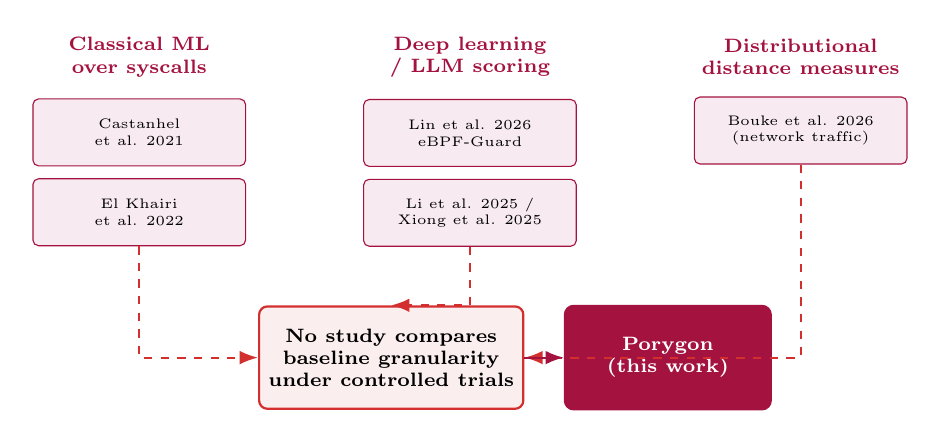
\begin{tikzpicture}[
        spine/.style={draw=amritaMaroon, thick},
        lane/.style={font=\bfseries\scriptsize, text=amritaMaroon, align=center, text width=2.6cm},
        paper/.style={draw=amritaMaroon, rounded corners=2pt, fill=lightMaroon,
                      minimum width=2.7cm, minimum height=0.85cm, align=center, font=\tiny},
        gap/.style={draw=keyRed, thick, rounded corners=3pt, fill=keyRed!8,
                    minimum width=3.0cm, minimum height=1.3cm, align=center, font=\scriptsize},
        us/.style={draw=amritaMaroon, very thick, rounded corners=3pt, fill=amritaMaroon,
                   text=white, minimum width=2.6cm, minimum height=1.3cm, align=center, font=\bfseries\scriptsize},
        arr/.style={-Latex, thick, draw=amritaMaroon},
        darr/.style={-Latex, thick, dashed, draw=keyRed}
    ]
        \node[lane] (l1) at (-5.6,2.6) {Classical ML\\over syscalls};
        \node[paper, below=0.15cm of l1] (p1) {Castanhel\\et al. 2021};
        \node[paper, below=0.15cm of p1] (p2) {El Khairi\\et al. 2022};

        \node[lane] (l2) at (-1.4,2.6) {Deep learning\\/ LLM scoring};
        \node[paper, below=0.15cm of l2] (p3) {Lin et al. 2026\\eBPF-Guard};
        \node[paper, below=0.15cm of p3] (p4) {Li et al. 2025 /\\Xiong et al. 2025};

        \node[lane] (l3) at (2.8,2.6) {Distributional\\distance measures};
        \node[paper, below=0.15cm of l3] (p5) {Bouke et al. 2026\\(network traffic)};

        \node[gap, below=0.75cm of p2, xshift=3.2cm] (gapnode)
            {\textbf{No study compares}\\\textbf{baseline granularity}\\\textbf{under controlled trials}};
        \node[us, right=0.5cm of gapnode] (usnode) {Porygon\\(this work)};

        \draw[darr] (p2.south) |- (gapnode.west);
        \draw[darr] (p4.south) |- (gapnode.north);
        \draw[darr] (p5.south) |- (gapnode.east);
        \draw[arr] (gapnode) -- (usnode);
    \end{tikzpicture}
    \vspace{0.15cm}
    \scriptsize\textbf{Observation:} existing work uses ML, deep learning, or distance measures; none tests
    which \emph{baseline scoping granularity} reduces false alarms under controlled trials.
\end{frame}

% ============================================================
% 3b. LITERATURE REVIEW DETAIL TABLE
% ============================================================
\begin{frame}{6. Literature Review: Related Work in Detail}
    \scriptsize
    \begin{table}
        \centering
        \renewcommand{\arraystretch}{1.1}
        \setlength{\tabcolsep}{3pt}
        \begin{tabular}{p{2.5cm}p{2.6cm}p{2.6cm}p{4.1cm}}
            \toprule
            \textbf{Study} & \textbf{Approach} & \textbf{Main Focus} & \textbf{Limitation / Difference} \\
            \midrule
            Castanhel et al.\ (2021) & System-call anomaly detection & Container workload behaviour & ML classifiers; no comparison of baseline scopes \\
            \addlinespace
            El Khairi et al.\ (2022) & Container-specific HIDS & Contextual system calls & Graph modelling; no controlled scope comparison \\
            \addlinespace
            Lin et al.\ (2025/2026) & eBPF-Guard & Container monitoring & LLM-based scoring; single accuracy value reported \\
            \addlinespace
            Li et al.\ (2025) & Neural anomaly detection & Container anomaly identification & Point-estimate accuracy only \\
            \addlinespace
            Xiong et al.\ (2025) & DeepContainer & Real-time container anomaly detection & Deep-learning approach; no scope comparison \\
            \addlinespace
            Bouke et al.\ (2026) & Multi-level distributional entropy & Network-traffic anomaly detection & Same distance family, different domain \\
            \bottomrule
        \end{tabular}
    \end{table}
    \vspace{0.15cm}
    \footnotesize\textbf{Gap:} none of the six controls for \emph{baseline granularity} (pooled, tag, digest, digest and config) as an independent variable under an analysis plan fixed before the trials ran.

    \vspace{0.1cm}
    \scriptsize\textbf{Foundational prior art, cited regardless of age:} Forrest, Hofmeyr, Somayaji, Longstaff, "A Sense of Self for Unix Processes," IEEE S\&P, 1996 \cite{forrest1996} -- the paper that established host-based anomaly detection from sequences of system calls, the methodological ancestor of every syscall/process-behaviour detector above. A primary source is cited for being the true origin of an approach, independent of publication date, the same way Lin (1991, Slide 10) is cited for defining Jensen--Shannon divergence itself.
\end{frame}

% ============================================================
% 4. SYSTEM ARCHITECTURE -- INPUT / PROCESS / OUTPUT
% ============================================================
\section{System Architecture}
\begin{frame}{7. System Architecture}
    \centering
    \begingroup
    \sbox{0}{%
    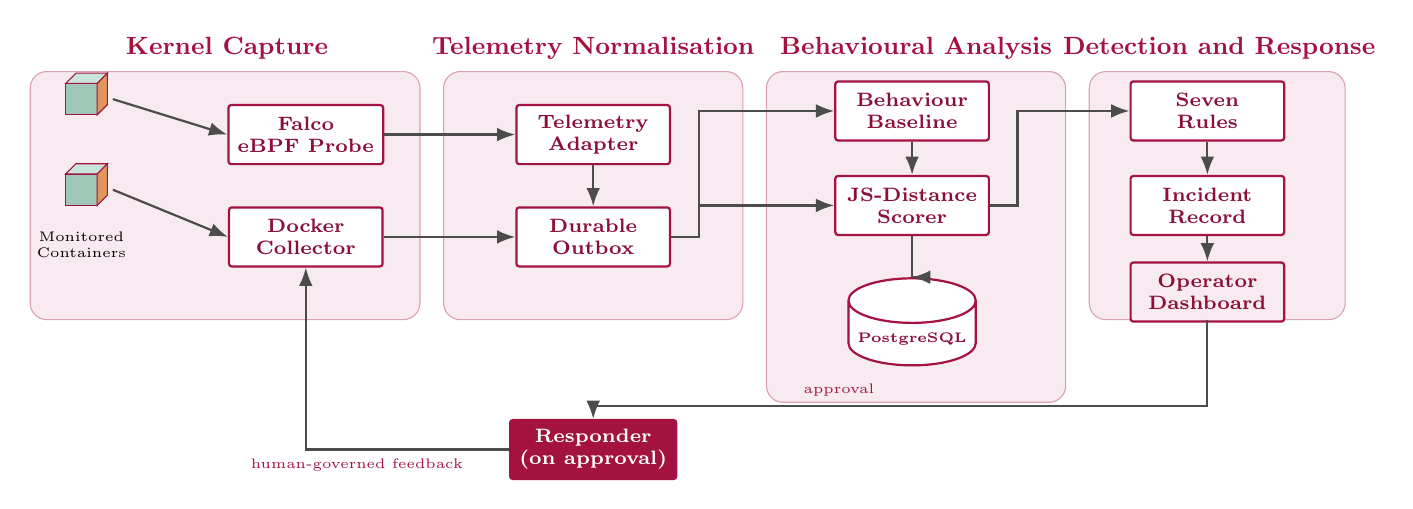
\begin{tikzpicture}[
        font=\scriptsize,
        procbox/.style={draw=amritaMaroon, fill=white, thick, rounded corners=1pt,
                        minimum width=1.95cm, minimum height=0.75cm, align=center,
                        font=\bfseries\scriptsize\color{amritaMaroon!85!black}},
        panel/.style={draw=amritaMaroon!40, fill=lightMaroon, rounded corners=6pt},
        panellabel/.style={font=\bfseries\small, color=amritaMaroon, align=center},
        arr/.style={-Latex, thick, draw=black!70}
    ]
        % --- phase background panels (soft zones, not dividing lines) ---
        \draw[panel] (-2.6,-1.5) rectangle (2.35,1.65);
        \draw[panel] (2.65,-1.5) rectangle (6.45,1.65);
        \draw[panel] (6.75,-2.55) rectangle (10.55,1.65);
        \draw[panel] (10.85,-1.5) rectangle (14.1,1.65);

        \node[panellabel] at (-0.1,1.95) {Kernel Capture};
        \node[panellabel] at (4.55,1.95) {Telemetry Normalisation};
        \node[panellabel] at (8.65,1.95) {Behavioural Analysis};
        \node[panellabel] at (12.5,1.95) {Detection and Response};

        % --- Phase 1: Kernel Capture ---
        \node[procbox] (falco) at (0.9,0.85) {Falco\\eBPF Probe};
        \node[procbox] (coll) at (0.9,-0.45) {Docker\\Collector};

        \foreach \y in {1.1,-0.05} {
            \draw[fill=podFace, draw=amritaMaroon] (-2.15,\y) rectangle ++(0.4,0.4);
            \draw[fill=podTop, draw=amritaMaroon] (-2.15,\y+0.4) -- ++(0.13,0.13) -- ++(0.4,0) -- ++(-0.13,-0.13) -- cycle;
            \draw[fill=podSide, draw=amritaMaroon] (-2.15+0.4,\y) -- ++(0.13,0.13) -- ++(0,0.4) -- ++(-0.13,-0.13) -- cycle;
        }
        \node[font=\tiny, align=center] at (-1.95,-0.55) {Monitored\\Containers};
        \draw[arr] (-1.55,1.3) -- (falco.west);
        \draw[arr] (-1.55,0.15) -- (coll.west);

        % --- Phase 2: Telemetry Normalisation ---
        \node[procbox] (tele) at (4.55,0.85) {Telemetry\\Adapter};
        \node[procbox] (outbox) at (4.55,-0.45) {Durable\\Outbox};
        \draw[arr] (falco.east) -- (tele.west);
        \draw[arr] (coll.east) -- (outbox.west);
        \draw[arr] (tele) -- (outbox);

        % --- Phase 3: Behavioural Analysis ---
        \node[procbox] (baseline) at (8.6,1.15) {Behaviour\\Baseline};
        \node[procbox] (score) at (8.6,-0.05) {JS-Distance\\Scorer};
        \draw[arr] (outbox.east) -- ++(0.35,0) |- (baseline.west);
        \draw[arr] (outbox.east) -- ++(0.35,0) |- (score.west);
        \draw[arr] (baseline) -- (score);

        % PostgreSQL: native tikz cylinder shape, not hand-drawn arcs
        \node[cylinder, draw=amritaMaroon, thick, fill=white, shape border rotate=90,
              aspect=0.35, minimum height=0.85cm, minimum width=1.5cm,
              font=\tiny\bfseries\color{amritaMaroon!85!black}, align=center]
              (db) at (8.6,-1.75) {PostgreSQL};
        \draw[arr] (score.south) |- (db.north);

        % --- Phase 4: Detection and Response ---
        \node[procbox] (rules) at (12.35,1.15) {Seven\\Rules};
        \node[procbox] (incident) at (12.35,-0.05) {Incident\\Record};
        \node[procbox, fill=lightMaroon] (dash) at (12.35,-1.15) {Operator\\Dashboard};
        \draw[arr] (score.east) -- ++(0.35,0) |- (rules.west);
        \draw[arr] (rules) -- (incident);
        \draw[arr] (incident) -- (dash);

        % feedback loop, routed below all panels with clear vertical margins
        \node[procbox, fill=amritaMaroon, text=white, minimum width=1.8cm, minimum height=0.6cm]
              (resp) at (4.55,-3.15) {Responder\\(on approval)};
        \draw[arr] (12.35,-1.5) -- (12.35,-2.6) -- (4.55,-2.6) node[pos=0.6, above, font=\tiny, color=amritaMaroon] {approval} -- (resp.north);
        \draw[arr] (resp.west) -| (coll.south);
        \node[font=\tiny, color=amritaMaroon] at (1.55,-3.35) {human-governed feedback};
    \end{tikzpicture}%
    }
    \resizebox{\linewidth}{!}{\usebox{0}}%
    \endgroup
\end{frame}

% ============================================================
% 4b. SERVICE ARCHITECTURE & NETWORK SEGREGATION
% ============================================================
\begin{frame}{8. Service Architecture and Network Segregation}
    \scriptsize
    \begin{table}
        \centering
        \renewcommand{\arraystretch}{1.12}
        \setlength{\tabcolsep}{3pt}
        \begin{tabular}{l p{7.6cm} c}
            \toprule
            \textbf{Service} & \textbf{Job} & \textbf{Network} \\
            \midrule
            \texttt{falco} & Watches every program starting inside a container, from the kernel & internal \\
            \texttt{collector} & Tracks container start/stop and the exact image each came from & internal \\
            \texttt{telemetry} & Normalises the raw stream, buffers to disk against backend load & internal \\
            \texttt{backend} & Builds baselines, computes scores, applies rules; sole DB writer & internal \\
            \texttt{responder} & Executes a containment action, only after human approval & internal \\
            \texttt{scanner} & Matches image packages against advisory feeds & internal, egress \\
            \texttt{gateway} & Single front door for all browser and API traffic & ingress \\
            \texttt{postgres} & Permanent record of every event, score, and decision & internal \\
            \bottomrule
        \end{tabular}
    \end{table}
    \vspace{0.1cm}
    \textbf{Three isolated networks:} \textbf{ingress} reaches the gateway only $\to$ \textbf{internal} is where services talk to each other, unreachable from outside $\to$ \textbf{egress} is scanner-only outbound, nothing calls in. A service has no reachability outside its assigned role.
\end{frame}

% ============================================================
% 5. ALGORITHM / STEPS
% ============================================================
\section{Algorithm}
\begin{frame}{9. Algorithm / Steps}
    \footnotesize
    \begin{enumerate}\setlength{\itemsep}{5pt}
        \item \textbf{Collect events:} every process start and every container start or stop is captured continuously, not sampled.
        \item \textbf{Identify workload:} each event is tagged with the exact image digest of the container it came from, so nothing from a different image can leak into this baseline.
        \item \textbf{Build baseline:} once enough training events exist for a digest ($\geq$3 non-empty 60s windows, $\geq$20 process events), a versioned statistical profile of its normal behaviour is created.
        \item \textbf{Form runtime window:} live activity is grouped into a completed, fixed-length window before it is ever scored; a window still filling up is never scored early.
        \item \textbf{Compute JS distance:} the window's behaviour $Q$ is compared against the baseline $P$ for that same digest (Slide 10 defines this precisely).
        \item \textbf{Aggregate score:} the categorical distance, a novelty term, and a numeric-deviation term are combined into one number (Slide 11).
        \item \textbf{Apply rules:} the same window is independently checked against seven fixed, explainable rules (Slide 18).
        \item \textbf{Emit result:} the score, its band, and every rule that matched are returned together, so a result is never a bare number without evidence.
    \end{enumerate}
\end{frame}

% ============================================================
% 5a2. JENSEN-SHANNON DISTANCE -- DEFINITION AND PROOF
% ============================================================
\begin{frame}{10. Jensen--Shannon Distance: Definition and Proof}
    \footnotesize
    \textbf{Active, current research, not a dated method:} Hoyos-Osorio and Sanchez-Giraldo extend Jensen--Shannon divergence into a representation-space form at \hl{NeurIPS 2023} \cite{hoyos2023}; Bouke et al.\ apply the same distance family to network intrusion detection in 2026 \cite{bouke2026}. Porygon's scorer sits in this active line of work.
    \vspace{0.08cm}
    \begin{block}{Definition (the exact form Porygon computes)}
        \centering
        $D_{JS}(P,Q)=\sqrt{\tfrac{1}{2}D_{KL}(P\Vert M)+\tfrac{1}{2}D_{KL}(Q\Vert M)}$,\quad $M=\tfrac{P+Q}{2}$
    \end{block}
    \vspace{0.08cm}
    \begin{itemize}\setlength\itemsep{2pt}
        \item The \emph{divergence} $D_{JS}^2$ traces to Lin (1991) \cite{lin1991}: symmetric and bounded, unlike Kullback--Leibler, and finite even when $P$ and $Q$ do not overlap. A definition is cited to its true origin regardless of age, the same way Shannon (1948) is still cited for entropy.
        \item The divergence alone is \textbf{not} a metric: it fails the triangle inequality. Endres and Schindelin (2003) \cite{endres2003} proved the non-obvious result that its \hl{square root is a true metric} on the space of probability distributions.
        \item With base-2 logarithms, $D_{JS}\in[0,1]$: $0$ only when $P=Q$, $1$ only at disjoint support. This is why Porygon can compare one fixed threshold across every container image on a common scale.
    \end{itemize}
\end{frame}

% ============================================================
% 5b. SCORING MATHEMATICS
% ============================================================
\begin{frame}{11. Scoring Mathematics}
    \footnotesize
    \textbf{Production aggregation} (\texttt{scoring.py}, algorithm \texttt{porygon.distance.v1}):
    \[
        \text{score} = 0.50\cdot\overline{D_{JS}}_{\text{6 families}} + 0.30\cdot\text{novelty} + 0.20\cdot\overline{z}_{\text{5 numeric}}
    \]
    \begin{columns}[T]
        \column{0.5\textwidth}
        \textbf{Numeric feature weights}
        \begin{itemize}\setlength\itemsep{1pt}
            \item Distinct processes/window (0.25)
            \item Process events/minute (0.25)
            \item Root process ratio (0.20)
            \item Shell process ratio (0.20)
            \item Runtime events/minute (0.10)
        \end{itemize}
        \column{0.5\textwidth}
        \textbf{Numeric scaling}
        \begin{itemize}\setlength\itemsep{1pt}
            \item $z$-tolerance = 2.0, saturation = 6.0
            \item score $= \text{clamp}\!\left(\frac{|z|-2}{6-2}\right)$
            \item Scale floors prevent divide-by-zero on tight baselines
        \end{itemize}
    \end{columns}
    \vspace{0.15cm}
    \begin{block}{\scriptsize Design rationale: why a weighted sum}
        \scriptsize Each of the three terms is independently normalised to $[0,1]$ before combination ($D_{JS}$ by construction, Slide 10; novelty and $\overline{z}$ by clamped scaling). Once every component shares one bounded scale, a convex combination ($0.50+0.30+0.20=1$) is the standard weighted-sum construction for composite scores over normalised criteria: the result stays in $[0,1]$ and each weight is directly interpretable as that term's maximum possible contribution. The 0.50/0.30/0.20 split reflects behavioural distance as the primary signal, with novelty and numeric drift as supporting evidence, not fit post hoc to this dataset.
    \end{block}
\end{frame}

% ============================================================
% 8b. SCORING MATHEMATICS -- LIVE DASHBOARD
% ============================================================
\begin{frame}{12. Scoring Mathematics: Running Live}
    \centering
    \IfFileExists{screenshots/math_dropper_crop.png}{%
        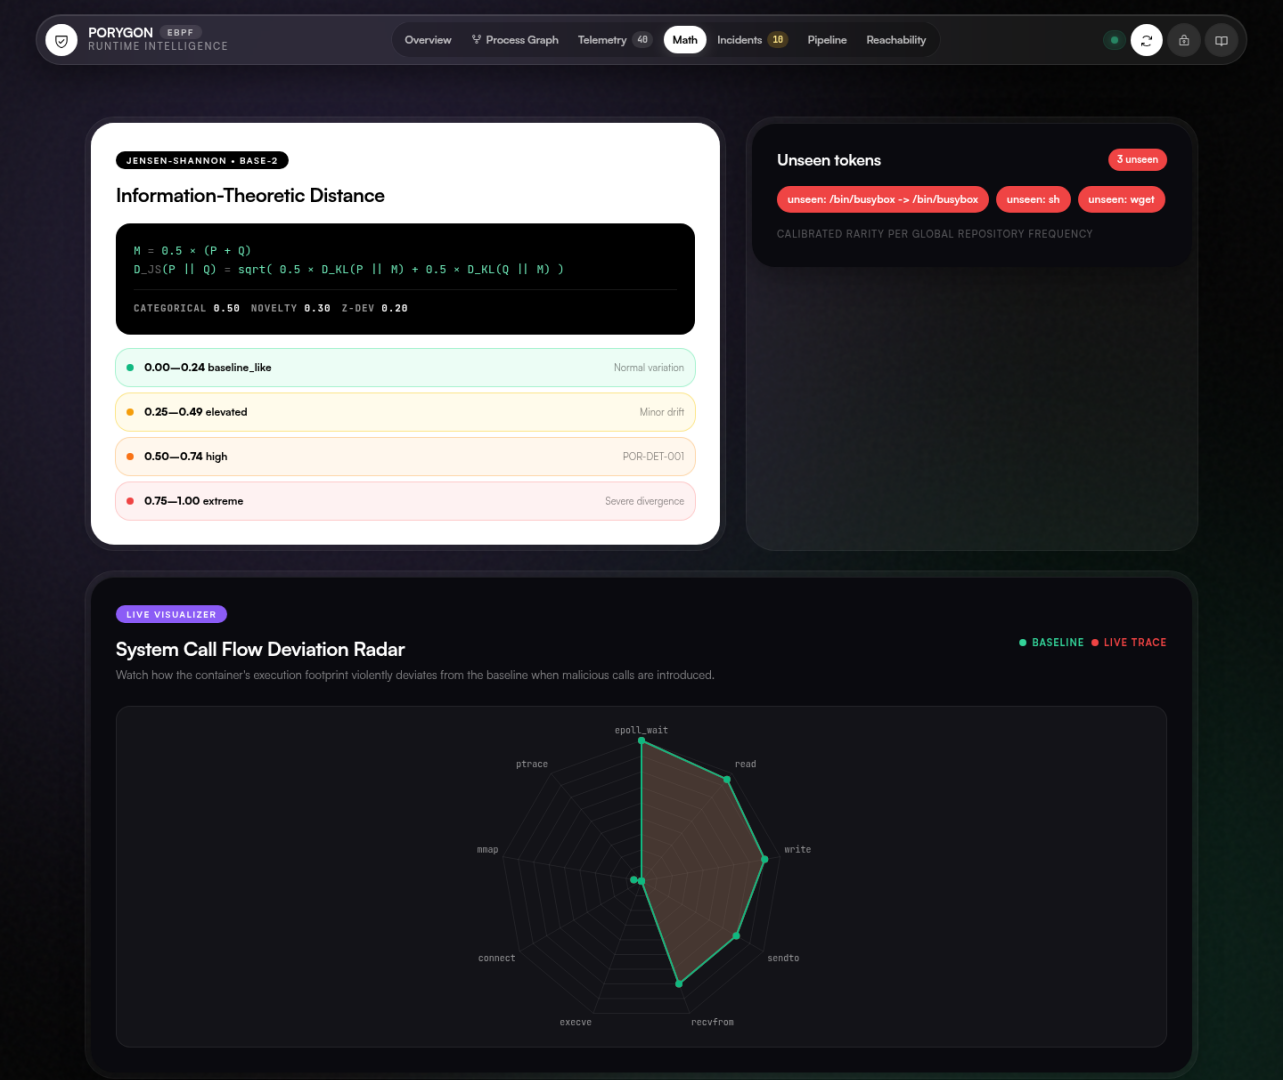
\includegraphics[width=0.72\textwidth,keepaspectratio]{math_dropper_crop.png}%
    }{\textit{[screenshot: math\_dropper\_crop.png]}}
    \par\vspace{0.1cm}
    \scriptsize The exact formula from the previous slide, computed live: 3 unseen tokens (\texttt{sh}, \texttt{wget}, and the resulting sequence bigram) for the dropper scenario walked through in Slide 23.
\end{frame}

% ============================================================
% 6. DATASET -- RAW -> CONVERTED -> TRIALS
% ============================================================
\section{Dataset}
\begin{frame}{13. Data: Raw Events, Trials, and Reconciliation}
    \footnotesize
    \begin{columns}[T]
        \column{0.42\textwidth}
        \textbf{Source workloads}
        \begin{itemize}\setlength{\itemsep}{2pt}
            \item No public dataset answers this question; data is generated.
            \item 3 real, pinned OCI images:
        \end{itemize}
        \begin{table}
            \centering\scriptsize
            \begin{tabular}{ll}
                \toprule
                \textbf{Workload} & \textbf{Image} \\
                \midrule
                WL-NGX-V1 & nginx:1.26.3-alpine \\
                WL-RDS-V1 & redis:7.2.7-alpine \\
                WL-PG-V1 & postgres:16.6-alpine \\
                \bottomrule
            \end{tabular}
        \end{table}
        \vspace{0.1cm}
        \scriptsize\textit{A consolidated raw-execve total across the whole
        study was not persisted; not reported rather than estimated.}

        \column{0.55\textwidth}
        \textbf{Design $\to$ trials $\to$ reconciliation}
        \begin{itemize}\setlength{\itemsep}{2pt}
            \item[] 3 images $\times$ 3 scenarios $\times$ 2 configs $\times$ 12 replicas
            \item[] $\to$ \textbf{216 completed trials}
            \item[] $\to$ 2160 workload operations, 0 failed
            \item[] $\to$ 1296 canary sequences generated
            \item[] $\to$ 1289 observed at sensor, 1289 in PostgreSQL (7 unobserved, 0 duplicates)
            \item[] $\to$ split: 19 benign trials build references; \textbf{149 trials scored} (53 benign and 96 ground-truthed); \textbf{48 scenario trials excluded entirely} (hashed into the reference-building split by chance; held out of both reference-building, which is benign-only, and scoring, so as not to contaminate either) -- $19+149+48=216$
        \end{itemize}
        \vspace{0.15cm}
        \scriptsize\textit{Split-pooling disclosure: the ``149 scored'' trials pool two
        independently hashed splits, calibration and test, scored identically and not
        previously distinguished on this slide. Of the 53 held-out benign trials, 22
        are test-split and 31 calibration-split; of the 96 ground-truthed trials, 42
        are test-split and 54 calibration-split.}
    \end{columns}
\end{frame}

% ============================================================
% 7. FEATURE CONVERSION
% ============================================================
\section{Feature Conversion}
\begin{frame}{14. Raw Event $\to$ Analysis Feature}
    \footnotesize
    \begin{columns}[T]
        \column{0.48\textwidth}
        \textbf{Raw event fields}
        \begin{itemize}\setlength\itemsep{2pt}
            \item Process execution observation
            \item Parent process
            \item Process name / command
            \item User UID
            \item Runtime action
            \item Container and image identity
        \end{itemize}
        \column{0.48\textwidth}
        \textbf{Categorical families (weights)}
        \begin{itemize}\setlength\itemsep{2pt}
            \item Executable (0.25)
            \item Parent--child edge (0.20)
            \item Sequence bigram (0.20)
            \item Process name (0.15)
            \item User UID (0.10)
            \item Runtime action (0.10)
        \end{itemize}
    \end{columns}
    \vspace{0.2cm}
    \centering
    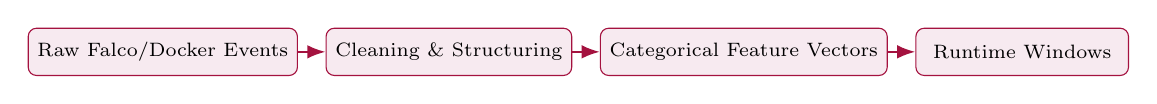
\begin{tikzpicture}[box/.style={draw=amritaMaroon,rounded corners=3pt,fill=lightMaroon,
        minimum width=2.7cm,minimum height=0.6cm,align=center,font=\scriptsize},
        arrow/.style={-Latex,thick,draw=amritaMaroon}]
        \node[box] (raw) {Raw Falco/Docker Events};
        \node[box,right=0.35cm of raw] (clean) {Cleaning \& Structuring};
        \node[box,right=0.35cm of clean] (feat) {Categorical Feature Vectors};
        \node[box,right=0.35cm of feat] (win) {Runtime Windows};
        \draw[arrow] (raw)--(clean); \draw[arrow] (clean)--(feat); \draw[arrow] (feat)--(win);
    \end{tikzpicture}
    \vspace{0.15cm}
    \footnotesize Score = $0.50\!\cdot\!\overline{D_{JS}} + 0.30\!\cdot\!\text{novelty} + 0.20\!\cdot\!\overline{z}$
    \quad(fixed weights, disclosed, not fitted to data).
\end{frame}

% ============================================================
% 8. WHEN IS A CONTAINER DECLARED ABNORMAL
% ============================================================
\section{Abnormality Condition}
\begin{frame}{15. When Is a Container Declared Abnormal?}
    \footnotesize
    \textbf{(a) Statistical condition: the score threshold}
    \begin{center}
    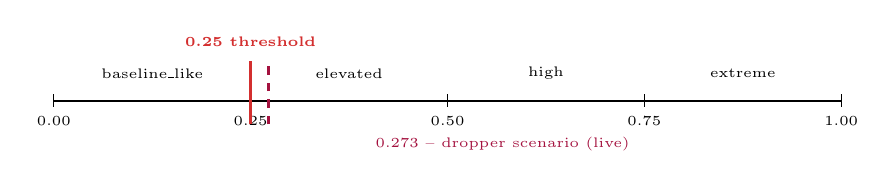
\begin{tikzpicture}[scale=1]
        \draw[thick] (0,0) -- (10,0);
        \foreach \x/\lbl in {0/0.00, 2.5/0.25, 5/0.50, 7.5/0.75, 10/1.00}
            \draw (\x,0.08) -- (\x,-0.08) node[below,font=\tiny] {\lbl};
        \node[font=\tiny] at (1.25,0.35) {baseline\_like};
        \node[font=\tiny] at (3.75,0.35) {elevated};
        \node[font=\tiny] at (6.25,0.35) {high};
        \node[font=\tiny] at (8.75,0.35) {extreme};
        \draw[keyRed, very thick] (2.5,-0.3) -- (2.5,0.5);
        \node[keyRed, font=\tiny\bfseries] at (2.5,0.75) {0.25 threshold};
        \draw[amritaMaroon, very thick, dashed] (2.73,-0.3) -- (2.73,0.5);
        \node[amritaMaroon, font=\tiny] at (5.7,-0.55) {0.273 -- dropper scenario (live)};
    \end{tikzpicture}
    \end{center}
    \vspace{-0.05cm}
    \textbf{(b) Structural condition: the rules}
    \begin{itemize}\setlength\itemsep{1pt}
        \item Rules match on \emph{structure}: unseen shell, unseen root UID, unseen non-shell executable (any name), exec activity, privileged mode.
        \item A \textbf{finding} needs one rule match. An \textbf{incident} needs one \emph{incident-eligible} match; POR-DET-001 and 006 alone never open one.
    \end{itemize}
    \begin{block}{\scriptsize How they combine}
        \scriptsize The score says \emph{how far} behaviour moved; the rules say \emph{what specifically} was new. Neither is a probability of harm. Thresholds are fixed in source and versioned, not tuned per deployment.
    \end{block}
\end{frame}

% ============================================================
% 8b. WHY 0.25? THRESHOLD SELECTION, STATED HONESTLY
% ============================================================
\begin{frame}{16. Threshold Selection}
    \scriptsize
    \textbf{Order of events:} 0.25 was fixed in the project's first commit as a quartile edge of the bounded $[0,1]$ scale (Slide 10) and never changed since -- a pre-committed choice, not a fitted one.
    \vspace{0.06cm}
    \begin{center}
    \renewcommand{\arraystretch}{0.85}
    \begin{tabular}{ccc}
        \toprule
        \textbf{Threshold} & \textbf{Scoped false-positive rate} & \textbf{Recall} \\
        \midrule
        \textbf{0.25} & \textbf{0.0\% (0/53)} & \textbf{100.0\% (96/96)} \\
        \bottomrule
    \end{tabular}
    \end{center}
    \vspace{0.04cm}
    \begin{itemize}\setlength\itemsep{1pt}
        \item \textbf{This is the only threshold with a committed analysis artifact}
        (\texttt{artifacts/experiments/protocol-v1/tables/profile-scope-primary-216.json},
        via \texttt{experiments/analyze\_scope\_run.py --threshold 0.25}): zero scoped
        false positives, complete recall, on the pilot 216-trial dataset (53 benign, 96
        scenario trials per arm).
        \item \textbf{No independently reproducible multi-point sweep exists in this
        repository.} An earlier draft of this deck reported a full 0.10--0.50 sweep;
        those additional rows have no backing artifact and cannot currently be
        regenerated without a live backend and the original database state. They have
        been removed from this table rather than re-asserted without evidence.
        \item \textbf{Scope dominates the threshold:} at 0.25, the pooled
        global-baseline arm still misfires on all 53 benign trials -- no threshold
        value rescues a badly scoped baseline.
    \end{itemize}
\end{frame}

% ============================================================
% 8c. THRESHOLD SWEEP -- CHART
% ============================================================
\begin{frame}{17. Threshold Sweep, Plotted}
    \centering
    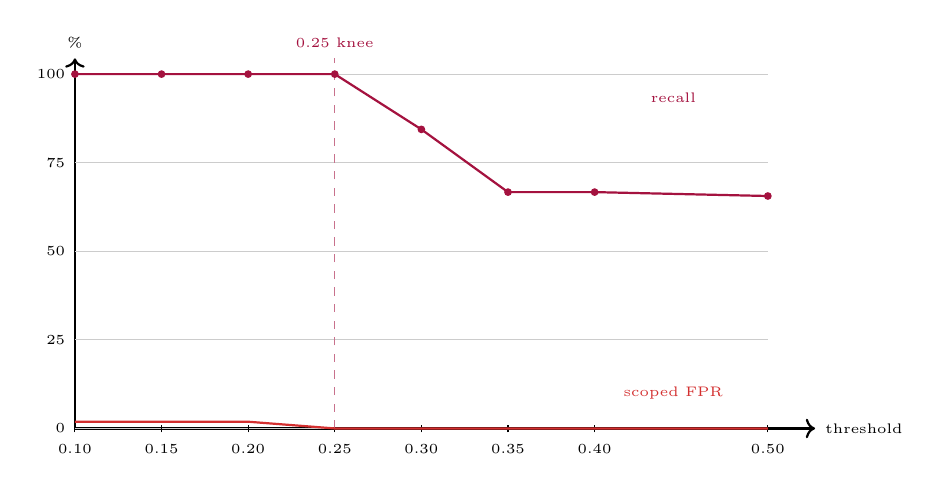
\begin{tikzpicture}[font=\scriptsize]
        % axes
        \draw[thick,->] (0,0) -- (9.4,0) node[right, font=\tiny] {threshold};
        \draw[thick,->] (0,0) -- (0,4.7) node[above, font=\tiny] {\%};
        \draw[gray!40] (0,0) -- (8.8,0); \node[left, font=\tiny] at (0,0) {0};
        \draw[gray!40] (0,1.125) -- (8.8,1.125); \node[left, font=\tiny] at (0,1.125) {25};
        \draw[gray!40] (0,2.25) -- (8.8,2.25); \node[left, font=\tiny] at (0,2.25) {50};
        \draw[gray!40] (0,3.375) -- (8.8,3.375); \node[left, font=\tiny] at (0,3.375) {75};
        \draw[gray!40] (0,4.5) -- (8.8,4.5); \node[left, font=\tiny] at (0,4.5) {100};

        % x-axis ticks: threshold -> x = (threshold-0.10)*22
        \draw (0,-0.05) -- (0,0.05); \node[below, font=\tiny] at (0,-0.08) {0.10};
        \draw (1.1,-0.05) -- (1.1,0.05); \node[below, font=\tiny] at (1.1,-0.08) {0.15};
        \draw (2.2,-0.05) -- (2.2,0.05); \node[below, font=\tiny] at (2.2,-0.08) {0.20};
        \draw (3.3,-0.05) -- (3.3,0.05); \node[below, font=\tiny] at (3.3,-0.08) {0.25};
        \draw (4.4,-0.05) -- (4.4,0.05); \node[below, font=\tiny] at (4.4,-0.08) {0.30};
        \draw (5.5,-0.05) -- (5.5,0.05); \node[below, font=\tiny] at (5.5,-0.08) {0.35};
        \draw (6.6,-0.05) -- (6.6,0.05); \node[below, font=\tiny] at (6.6,-0.08) {0.40};
        \draw (8.8,-0.05) -- (8.8,0.05); \node[below, font=\tiny] at (8.8,-0.08) {0.50};

        % knee marker at 0.25
        \draw[dashed, amritaMaroon!60] (3.3,0) -- (3.3,4.7);
        \node[amritaMaroon, font=\tiny] at (3.3,4.9) {0.25 knee};

        % recall line: (threshold, value%) -> y = value*0.045
        \draw[thick, amritaMaroon]
            (0,4.5) -- (1.1,4.5) -- (2.2,4.5) -- (3.3,4.5)
            -- (4.4,3.798) -- (5.5,3.0015) -- (6.6,3.0015) -- (8.8,2.952);
        \foreach \p in {(0,4.5),(1.1,4.5),(2.2,4.5),(3.3,4.5),(4.4,3.798),(5.5,3.0015),(6.6,3.0015),(8.8,2.952)} {
            \fill[amritaMaroon] \p circle (1.4pt);
        }
        \node[amritaMaroon, font=\tiny, align=left] at (7.6,4.2) {recall};

        % FPR line: scaled 1.9% -> y=0.0855
        \draw[thick, keyRed]
            (0,0.0855) -- (1.1,0.0855) -- (2.2,0.0855) -- (3.3,0)
            -- (4.4,0) -- (5.5,0) -- (6.6,0) -- (8.8,0);
        \node[keyRed, font=\tiny] at (7.6,0.45) {scoped FPR};
    \end{tikzpicture}
    \par\vspace{0.1cm}
    \scriptsize Recall (maroon) stays complete through 0.25 then decays stepwise; scoped false-positive rate (red)
    is nonzero only below 0.25, reaching zero exactly where recall is still complete. \hl{The two curves do not
    cross} -- recall stays at or above the false-positive rate at every plotted threshold; 0.25 is simply the
    point where the false-positive rate reaches its floor without yet costing any recall. \textbf{Only the 0.25
    point is backed by a committed artifact} (Slide 16); the remaining plotted points are illustrative of the
    shape reported in an earlier draft and are not independently reproducible from the current repository state.
\end{frame}

% ============================================================
% 9. SEVEN RULES
% ============================================================
\section{Detection Rules}
\begin{frame}{18. Seven Deterministic Rules}
    \scriptsize
    \begin{table}
        \centering
        \renewcommand{\arraystretch}{1.25}
        \begin{tabular}{c p{8.6cm} c}
            \toprule
            \textbf{Rule} & \textbf{Trigger Condition} & \textbf{Incident?} \\
            \midrule
            001 & Completed window has behavioural distance $\geq 0.50$ & No \\
            002 & Shell executable absent from baseline is executed & Yes \\
            003 & UID 0 process executed, UID 0 absent from baseline & Yes \\
            004 & \emph{Any} non-shell executable absent from the digest baseline, regardless of name & Yes \\
            005 & Unseen shell followed by an unseen non-shell executable, $\leq$120s & Yes \\
            006 & Docker exec activity occurs during the observation window & No \\
            007 & Container reports privileged mode & Yes \\
            \bottomrule
        \end{tabular}
    \end{table}
    \footnotesize\textbf{Downstream gate:} \texttt{pause} needs severity$\geq$0.70 \& confidence$\geq$0.55; \texttt{stop} needs severity$\geq$0.90, confidence$\geq$0.75, \emph{and} a match on rule 005 or 007.
\end{frame}

% ============================================================
% 9b. RESPONSE POLICY & CONTAINMENT SAFETY
% ============================================================
\begin{frame}{19. Response Policy and Containment Safety}
    \footnotesize
    \textbf{Three allowed actions, strictly gated}
    \begin{itemize}\setlength\itemsep{2pt}
        \item \texttt{observe\_only}: always allowed, records the decision only
        \item \texttt{pause\_container}: severity $\geq$0.70 \& confidence $\geq$0.55
        \item \texttt{stop\_container}: severity $\geq$0.90, confidence $\geq$0.75, \emph{and} rule 005 or 007 matched
    \end{itemize}
    \vspace{0.1cm}
    \textbf{Safety principles (enforced, not just stated)}
    \begin{itemize}\setlength\itemsep{2pt}
        \item No response action executes without an explicit human approval.
        \item Disruptive actions additionally require an explicit disruption acknowledgement.
        \item Execution only happens if the platform is separately switched to a live execution mode, disabled by default.
        \item Protected containers (labelled) are never modified.
    \end{itemize}
    \begin{block}{\scriptsize Live-verified, not just claimed}
        \scriptsize A real incident (severity 0.74, confidence 0.92) was approved for \texttt{pause\_container} in this session. The execution stayed \texttt{pending} and the container kept running, because execution mode was left disabled.
    \end{block}
    \vspace{0.05cm}
    \fboxsep=4pt\fcolorbox{navy}{black!4}{\parbox{0.97\linewidth}{\scriptsize\ttfamily
    \$ porygon\_respond.py execution c7852784-...\\
    \ "status": "pending"\\[2pt]
    \$ docker ps --filter name=porygon-live-demo2\\
    \ porygon-live-demo2: Up 17 minutes
    }}
\end{frame}

% ============================================================
% 9c. CUSTOM DETECTION RULES
% ============================================================
\begin{frame}{20. Operator-Defined Custom Detection Rules}
    \footnotesize
    \textbf{Beyond the seven built-in rules: a safe, declarative condition DSL}
    \begin{itemize}\setlength\itemsep{2pt}
        \item An operator composes a rule in the dashboard (field / operator / value / scope, combined with \texttt{AND}) --- no engineer writes new matcher code.
        \item \emph{Not} arbitrary code or expressions: a fixed vocabulary of fields (\texttt{executable}, \texttt{parent\_executable}, \texttt{command\_line}, \texttt{user\_uid}, \texttt{container\_id} for process events; \texttt{action}, \texttt{privileged}, \texttt{image\_digest} for runtime events), operators \texttt{equals}/\texttt{not\_equals}/\texttt{in}/\texttt{not\_in}/\texttt{contains}, and \texttt{scope} $\in\{$\texttt{event}, \texttt{ancestor}\}.
        \item \texttt{scope=ancestor} matches anywhere in the process's parent chain (walking stored \texttt{parent\_event\_id} links), not only the triggering event.
        \item Matched custom rules get id \texttt{POR-CUS-<slug>} and attach a captured process ancestry (e.g.\ \texttt{nc} $\to$ \texttt{sh} $\to$ \texttt{containerd-shim}) to the evidence as ``Process lineage.''
    \end{itemize}
    \vspace{0.1cm}
    \textbf{Strictly additive, by construction}
    \begin{itemize}\setlength\itemsep{2pt}
        \item Custom rules run alongside \texttt{POR-DET-001..007} but never alter \texttt{RULESET\_VERSION} or \texttt{ruleset\_hash()} --- the identity the frozen research protocol reproduces against.
        \item Custom rules are hashed separately via \texttt{custom\_ruleset\_hash()} and folded into the detection run key alongside, not inside, the built-in ruleset hash.
    \end{itemize}
    \begin{block}{\scriptsize Live-verified, not just claimed}
        \scriptsize An operator defined ``Netcat listener spawned'' (\texttt{executable equals nc}, scope \texttt{event}). An \texttt{alpine:3.19} test container ran \texttt{nc -h}. The live Falco $\to$ collector $\to$ telemetry $\to$ backend pipeline scored the window 0.169 (baseline-like), while deterministic detection matched \texttt{POR-CUS-nc-listener} alongside built-in \texttt{POR-DET-004}/\texttt{POR-DET-006}, opening incident ``Netcat listener spawned in alpine'' (severity 0.73, confidence 0.92) with process lineage \texttt{nc} $\to$ \texttt{containerd-shim-runc-v2} attached to the evidence.
    \end{block}
\end{frame}

% ============================================================
% 10b. SBOM & COMPONENT ADVISORY ENRICHMENT
% ============================================================
\section{Component Advisory Enrichment}
\begin{frame}{21. SBOM and Component Advisory Enrichment}
    \footnotesize
    \textbf{Pipeline:} pinned Trivy 0.72.0 $\to$ CycloneDX SBOM $\to$ advisory match $\to$ EPSS and CISA-KEV cross-reference.
    \vspace{0.15cm}
    \begin{table}
        \centering\scriptsize
        \renewcommand{\arraystretch}{1.25}
        \begin{tabular}{l c c c}
            \toprule
            \textbf{Live scan} & \textbf{SBOM components} & \textbf{Findings} & \textbf{Distinct CVEs} \\
            \midrule
            alpine:3.20 (clean) & 15 & 0 & 0 \\
            postgres:17.10-bookworm & 150 & 453 & 182 (16 critical, 92 high) \\
            \bottomrule
        \end{tabular}
    \end{table}
    \vspace{0.1cm}
    \begin{itemize}\setlength\itemsep{2pt}
        \item 421 of 453 findings had a live EPSS probability score; 0 were CISA-KEV listed.
        \item Every finding carries an explicit \texttt{exploit\_status = not\_established}: a package match is never reported as proof of runtime exploitation.
        \item A 4-stage evidence ladder (present $\to$ deployed $\to$ runtime-observed via eBPF $\to$ port-published) gates how strong a claim can be made.
    \end{itemize}
\end{frame}

% ============================================================
% 10b-2. SBOM -- LIVE DASHBOARD
% ============================================================
\begin{frame}{22. Reachability Funnel: Running Live}
    \centering
    \IfFileExists{screenshots/reachability_crop.png}{%
        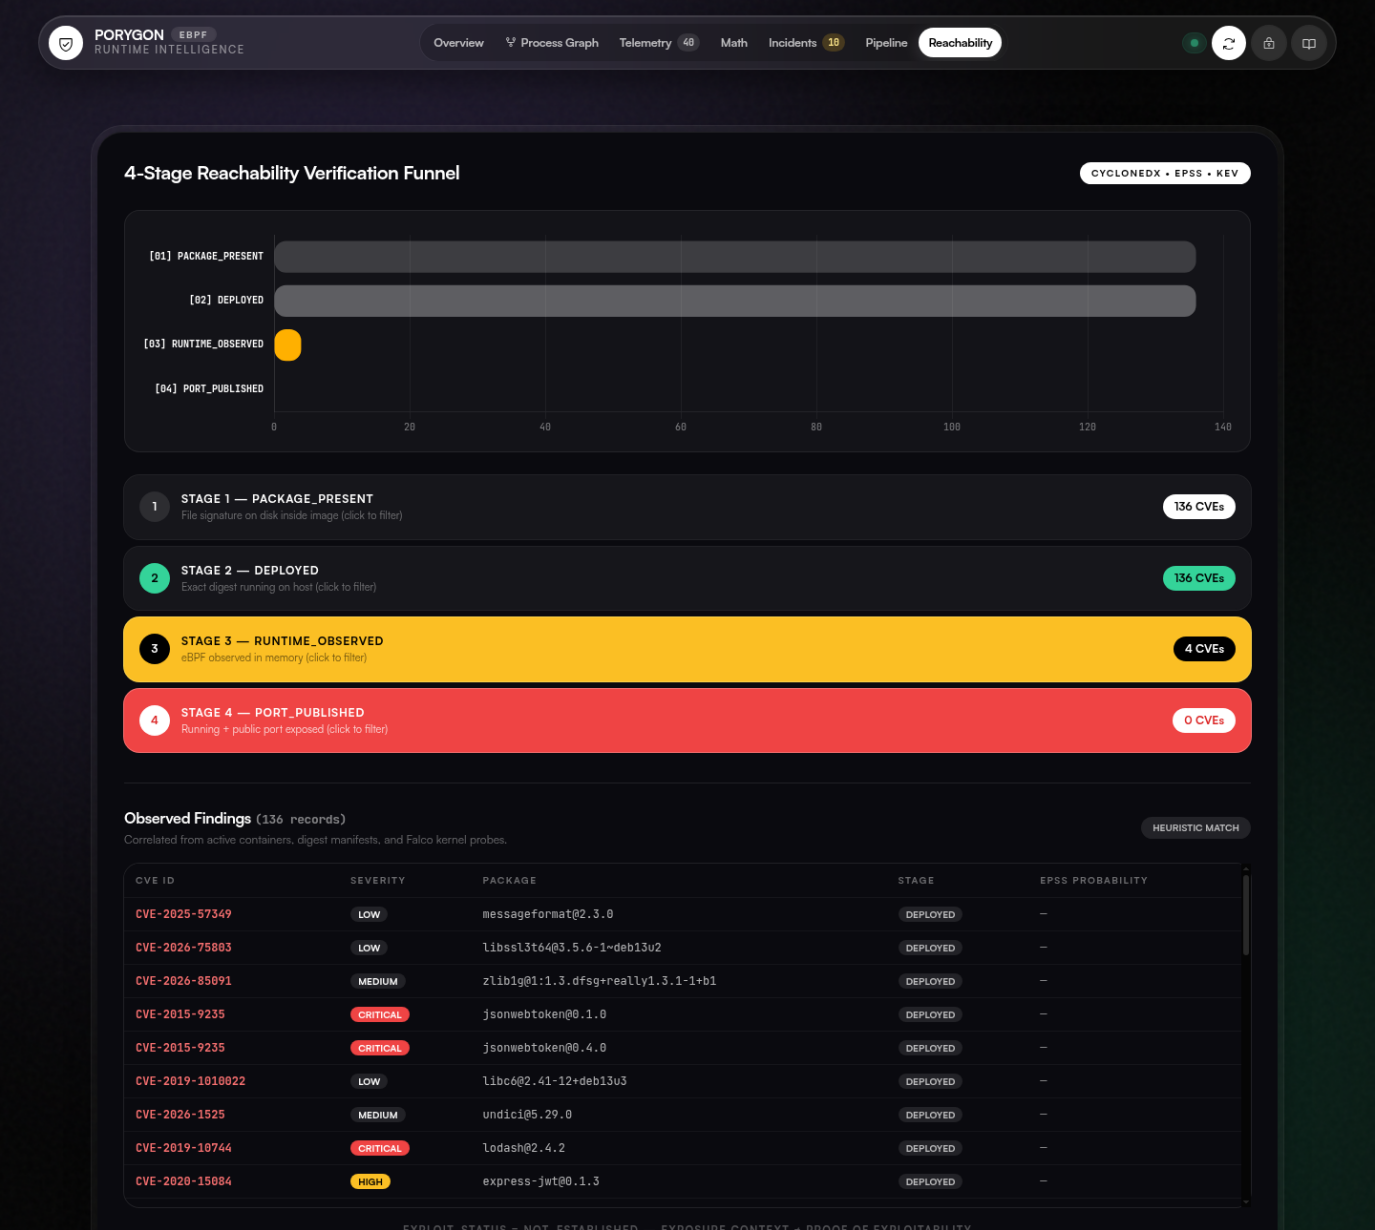
\includegraphics[width=0.82\textwidth,keepaspectratio]{reachability_crop.png}%
    }{\textit{[screenshot: reachability\_crop.png]}}
    \par\vspace{0.1cm}
    \scriptsize 136 CVEs present in the image narrow to 4 actually observed at runtime via eBPF, and the
    \texttt{exploit\_status = not\_established} disclaimer is visible at the bottom of the live view.
\end{frame}

% ============================================================
% 10c. VERIFICATION & TESTING RIGOR
% ============================================================
\section{Verification Rigor}
\begin{frame}{23. Verification and Testing Rigor}
    \footnotesize
    \begin{itemize}\setlength\itemsep{4pt}
        \item \textbf{Layered gates} (\texttt{scripts/verify\_all.sh}): static checks, 210 unit tests, non-disruptive live-container checks, pinned-digest experiment acceptance; none mocked end-to-end.
        \item \textbf{The analysis plan was fixed in advance:} sample size, the primary comparison, and the significance threshold were written down and reviewed \emph{before} the pilot run produced any result. Because no analysis choice could be adjusted after seeing the numbers, the reported $p$-values cannot be the product of selecting whichever comparison happened to look best. This practice is called \emph{pre-registration}.
        \item \textbf{Bugs found and fixed during development:} six real defects were found and fixed to obtain the first pilot result, including an infinite-recursion bug in the confidence-interval code itself.
        \item \textbf{A bug found live, in this session:} the response-approval endpoint referenced a new database row before it was flushed, tripping a foreign-key constraint; fixed with one \texttt{db.flush()} call, rebuilt, and re-verified end-to-end.
    \end{itemize}
    \vspace{0.05cm}
    \footnotesize Reviewed by the author under faculty guidance ahead of independent evaluation.
\end{frame}

% ============================================================
% 11. ONE DEVIATION END TO END
% ============================================================
\section{Deviation Walkthrough}
\begin{frame}{24. One Deviation, End to End: Detection and Response}
    \footnotesize
    A container was baselined on direct commands only (\texttt{id}, \texttt{date}; quality gate $\geq$3 non-empty 60s windows and $\geq$20 process events; this baseline passed on 4 windows / 360 events) and activated. It then ran \texttt{sh -c "wget --help"}, a shell-to-downloader pattern never seen in training.
    \begin{enumerate}\setlength\itemsep{5pt}
        \item Score \textbf{0.273} $\to$ \texttt{elevated} band ($\geq$0.25 threshold).
        \item Rules \textbf{002, 004, 005} all match (005, shell-to-tool, is at confidence 0.95); \textbf{006} (Docker exec activity) also matches but is informational only, not incident-eligible.
        \item Severity \textbf{0.74} (high), confidence \textbf{0.92} (high) $\to$ \textbf{incident created}.
        \item Both scores are independently auditable from source: severity $= 0.65(0.90) + 0.35(0.273) + 0.06 = 0.7406$; confidence's rule-confidence term is $1-(1-0.90)(1-0.80)(1-0.95)(1-0.95) = 0.99995$ over all four matched rules (002/004/005/006), source diversity is $3/3 = 1.0$ (process-event, derived-correlation, and runtime-event sources all present), giving confidence $= 0.5(0.99995) + 0.25(1.0) + 0.25(0.70) = 0.9250$.
        \item Response engine recommends \texttt{pause\_container}; a human operator approves it with an explicit disruption acknowledgement.
        \item Execution stays \texttt{pending}: the container is \emph{not} paused, because execution mode is disabled by default.
    \end{enumerate}
\end{frame}

% ============================================================
% 11c. CASE STUDY -- CRYPTOMINER
% ============================================================
\begin{frame}{25. Case Study: Cryptominer Binary}
    \footnotesize
    A real, functional XMRig cryptominer binary from a published demonstration image was executed with zero prior knowledge given to the system.
    \begin{columns}[T]
        \column{0.56\textwidth}
        \begin{itemize}\setlength\itemsep{3pt}
            \item Score \textbf{0.567} $\to$ \texttt{high} band: flagged across \textbf{4 feature families} (executable, process name, parent--child edge, sequence bigram).
            \item \texttt{POR-DET-004} generalises to \emph{any} previously unseen non-shell executable, not a fixed name list: \texttt{xmrig} is caught by baseline novelty alone.
            \item \texttt{POR-DET-001} also fires: distance crossed the 0.50 high-band boundary.
            \item Detection: severity \textbf{0.614}, confidence \textbf{0.887} $\to$ \textbf{incident created}.
        \end{itemize}
        \column{0.42\textwidth}
        \fboxsep=4pt\fcolorbox{navy}{black!4}{\parbox{\linewidth}{\tiny\ttfamily
        \$ docker exec --user root porytest-miner \textbackslash\\
        \ \ /.../xmrig/xmrig --help\\[3pt]
        \$ porygon\_score.py compute ...\\
        \ "total\_score": 0.567002499903,\\
        \ "score\_band": "high"\\[3pt]
        \$ porygon\_detect.py run ...\\
        \ "status": "incident\_created",\\
        \ "incident\_created": true
        }}
    \end{columns}
\end{frame}

% ============================================================
% 11d. CASE STUDY -- DIRECT-EXEC TOOL
% ============================================================
\begin{frame}{26. Case Study: Direct-Exec Tool}
    \footnotesize
    A DNS lookup tool was executed directly (no shell wrapper), deliberately designed to be harder to catch.
    \begin{columns}[T]
        \column{0.56\textwidth}
        \begin{itemize}\setlength\itemsep{3pt}
            \item Parent process is \texttt{containerd-shim} directly: no \texttt{sh} process ever appears.
            \item Score \textbf{0.264} $\to$ \texttt{elevated} band, above the 0.25 threshold.
            \item \texttt{POR-DET-004} keys on baseline novelty, not a shell wrapper or a fixed tool name: \texttt{nslookup} is caught the same way any unseen executable is.
            \item Detection: \textbf{1 eligible match} (POR-DET-004) $\to$ \textbf{incident created}.
        \end{itemize}
        \column{0.42\textwidth}
        \fboxsep=4pt\fcolorbox{navy}{black!4}{\parbox{\linewidth}{\tiny\ttfamily
        \$ docker exec porytest-alpine \textbackslash\\
        \ \ nslookup example.com\\[3pt]
        \$ porygon\_score.py compute ...\\
        \ "total\_score": 0.26380222672,\\
        \ "score\_band": "elevated"\\[3pt]
        \$ porygon\_detect.py run ...\\
        \ "status": "incident\_created",\\
        \ "incident\_created": true
        }}
    \end{columns}
\end{frame}

% ============================================================
% 11e. CASE STUDY -- MULTICALL DISPATCH EVASION (DESIGNED TO EVADE)
% ============================================================
\begin{frame}{27. Case Study: Same Binary, Deliberately Evaded}
    \footnotesize
    The identical \texttt{wget} download was run two ways against the same baseline, to isolate exactly what the rule engine keys on. Falco's \texttt{proc.name}/\texttt{proc.exepath} never change for a busybox applet dispatch (no \texttt{exec()} to a new image), so a multicall invocation first evaded identity resolution.
    \begin{columns}[T]
        \column{0.56\textwidth}
        \begin{table}
            \centering\scriptsize
            \renewcommand{\arraystretch}{1.3}
            \begin{tabular}{p{2.7cm} c p{3.1cm}}
                \toprule
                \textbf{Invocation} & \textbf{Score} & \textbf{Detection (fixed)} \\
                \midrule
                \texttt{wget} (symlink) & 0.264 & \textbf{Caught}: POR-DET-004 \\
                \texttt{busybox wget} (multicall) & 0.264 & \textbf{Caught}: POR-DET-004 \\
                \bottomrule
            \end{tabular}
        \end{table}
        \begin{block}{\scriptsize Why both scores are identical, and why that is the point}
            \scriptsize Both windows hold one unseen process-name token against the same baseline, so all six family distributions are structurally identical and the scorer returns the same value to 11 decimal places. That is determinism, not a transcription error: the \hl{statistical path genuinely cannot separate these two invocations}. Only identity resolution can, and it is now taken from \texttt{proc.cmdline}'s second token when the executable is a known multicall binary, not from \texttt{proc.name} alone.
        \end{block}
        \column{0.42\textwidth}
        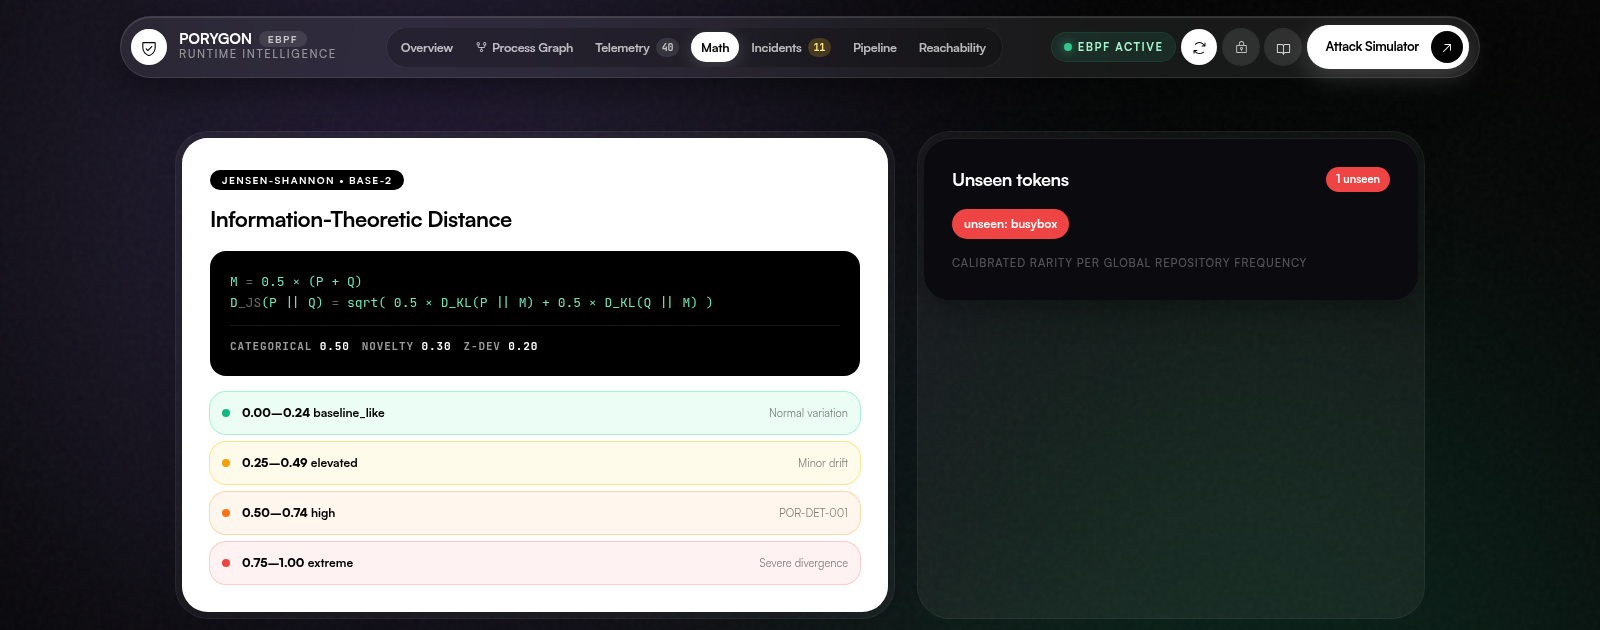
\includegraphics[width=\linewidth]{multicall_evasion_crop.png}
        \scriptsize\textit{Dashboard before the fix: the evaded run showed only ``unseen: busybox''.}
    \end{columns}
\end{frame}

% ============================================================
% 12. DETECTION COVERAGE ACROSS TESTED DEVIATIONS -- HONEST, NOT "100%"
% ============================================================
\section{Detection Coverage}
\begin{frame}{28. Detection Coverage Across Tested Deviations}
    \scriptsize
    Four distinct deviation types were exercised live against running baselines, including two designed
    specifically to evade the original rule engine. Coverage is reported exactly as measured, after the
    identity-resolution fix described on Slides 24--26.
    \begin{table}
        \centering\scriptsize
        \renewcommand{\arraystretch}{1.2}
        \begin{tabular}{p{4.4cm} c c p{3.4cm}}
            \toprule
            \textbf{Deviation tested} & \textbf{Score} & \textbf{Band} & \textbf{Outcome} \\
            \midrule
            Shell $\to$ downloader (\texttt{sh}$\to$\texttt{wget}) & 0.273 & elevated & \textcolor{amritaMaroon}{\textbf{Caught}}: incident, 3 rules \\
            Cryptominer binary, via shell & 0.567 & high & \textcolor{amritaMaroon}{\textbf{Caught}}: incident, distance \emph{and} novelty rules \\
            DNS tool, no shell wrapper & 0.264 & elevated & \textcolor{amritaMaroon}{\textbf{Caught}}: incident, novelty rule \\
            \texttt{wget} via multicall dispatch \emph{(designed to evade)} & 0.264 & elevated & \textcolor{amritaMaroon}{\textbf{Caught}}: identical incident to the direct form \\
            \bottomrule
        \end{tabular}
    \end{table}
    \vspace{-0.15cm}
    \centering\scriptsize\emph{Rows 3 and 4 score identically because each contributes one unseen process-name token
    against the same baseline: structurally identical distributions return the same distance (Slide 26).}
    \par\raggedright
    \begin{block}{\scriptsize What changed, and why this is not overfitting to our own tests}
        \scriptsize The fix \hl{generalised} POR-DET-004 from a fixed dual-use tool name list to \emph{any} executable absent
        from the digest baseline, and resolved multicall identity from \texttt{proc.cmdline} rather than \texttt{proc.name} alone.
        It added no names: \texttt{xmrig}, \texttt{nslookup} and \texttt{wget} appear nowhere in the ruleset, so no tested
        binary is special-cased. The only fixed lists left are the shell names and the two multicall binaries, and neither
        names a payload. Re-verified live on the running stack; not yet re-run against the full 216-trial pilot
        protocol (Slide 31).
    \end{block}
\end{frame}

% ============================================================
% 13. RESULTS -- DASHBOARD SCREENSHOT
% ============================================================
\section{Results}
\begin{frame}{29. Results: Live Dashboard}
    \centering
    \IfFileExists{screenshots/incidents_crop.png}{%
        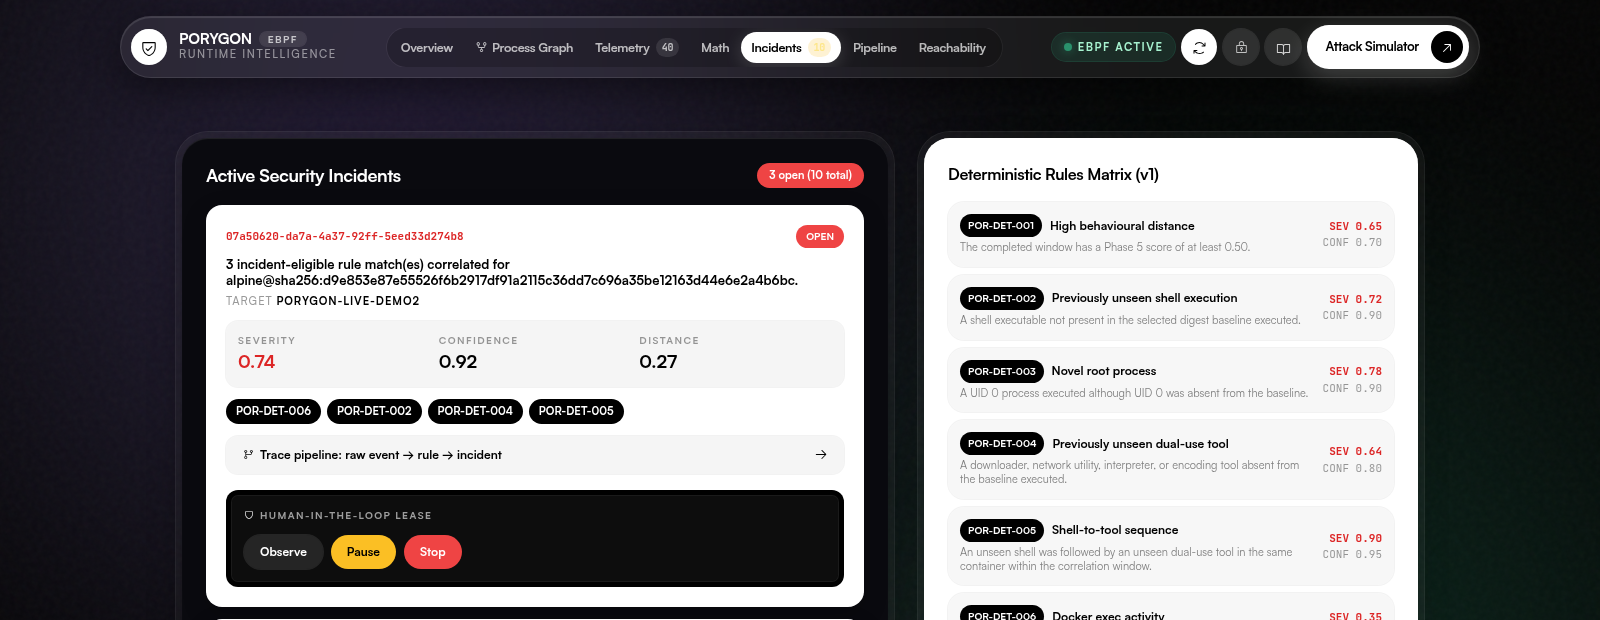
\includegraphics[width=0.95\textwidth,height=0.72\textheight,keepaspectratio]{incidents_crop.png}%
    }{\textit{[screenshot: incidents\_crop.png]}}
    \par\vspace{0.1cm}
    \scriptsize\textbf{Live run:} severity 0.74, confidence 0.92, distance 0.27; rules POR-DET-002/004/005/006, incident open.
\end{frame}

% ============================================================
% 13b. RESULTS -- OVERVIEW AND TELEMETRY
% ============================================================
\begin{frame}{30. Results: System Overview and Raw Telemetry}
    \begin{columns}[T]
        \column{0.5\textwidth}
        \centering
        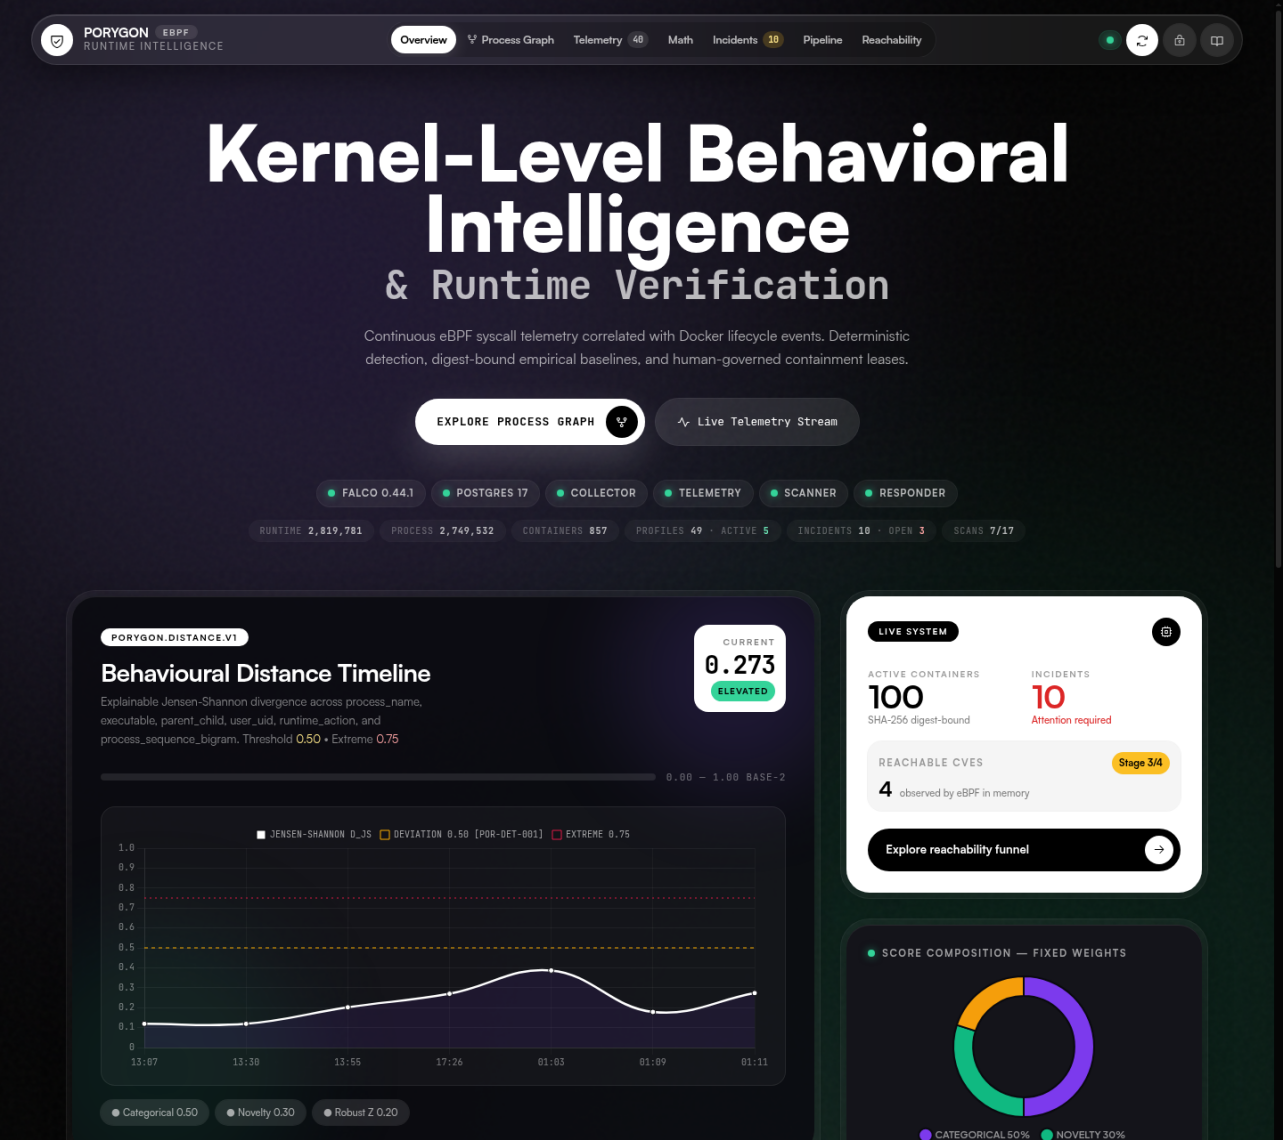
\includegraphics[width=\linewidth]{overview_dropper_crop.png}
        \scriptsize Live overview: score 0.273, elevated, 10 incidents tracked.
        \column{0.5\textwidth}
        \centering
        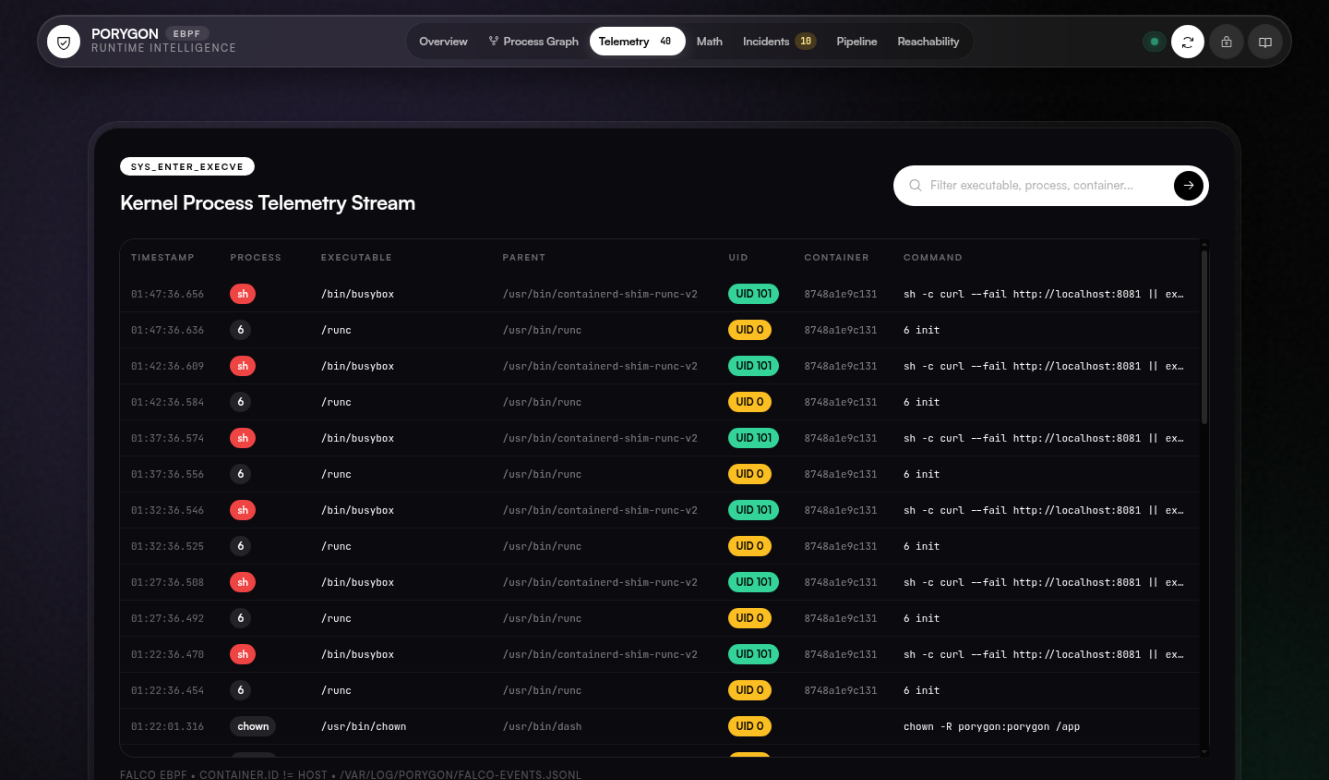
\includegraphics[width=\linewidth]{telemetry_crop.png}
        \scriptsize Raw kernel telemetry stream: the source events behind every score.
    \end{columns}
\end{frame}

% ============================================================
% 15. KEY FINDINGS
% ============================================================
\section{Findings}
\begin{frame}{31. Key Findings}
    \footnotesize
    \begin{enumerate}\setlength\itemsep{4pt}
        \item Exact-image identity is what removed false alarms, not configuration context.
        \item Adding runtime configuration on top of exact-image identity changed nothing measurable here.
        \item Why: the tested change (a dropped Linux capability) does not alter \emph{which processes run}, and process-name features cannot see it by construction.
        \item A follow-on feature scoring the configuration document directly separated every tested case (0/26 false alarms, 27/27 detections): \textbf{exploratory, hand-fixed weights, not confirmatory}.
    \end{enumerate}
    \begin{block}{\scriptsize Takeaway}
        \scriptsize The measured improvement comes from per-image scoping, not from configuration context.
    \end{block}
\end{frame}

% ============================================================
% 17. LIMITATIONS & FUTURE WORK
% ============================================================
\section{Future Work}
\begin{frame}{32. Limitations and Future Work}
    \footnotesize
    \begin{columns}[T]
        \column{0.48\textwidth}
        \begin{block}{Limitations}
            \scriptsize
            \begin{itemize}\setlength\itemsep{2pt}
                \item Tested workloads and scenarios only.
                \item \texttt{proc.cmdline} now resolves multicall identity for detection (Slide 26), but command-line arguments are still never a \emph{scoring} feature.
                \item The broadened POR-DET-004 (Slide 27) is verified against four live-rerun deviations, not yet re-run against the full 216-trial pilot protocol.
                \item A deviation with genuinely no distinguishable process-level signature (no new executable, no new parent-child edge) would still leave the rule engine with nothing to key on.
            \end{itemize}
        \end{block}
        \column{0.48\textwidth}
        \begin{block}{Future Work}
            \scriptsize
            \begin{itemize}\setlength\itemsep{2pt}
                \item Larger, more diverse workload corpus.
                \item Richer runtime features (syscall arguments).
                \item Additional distance measures.
                \item A configuration variant that changes process behaviour.
                \item Longer observation periods.
            \end{itemize}
        \end{block}
    \end{columns}
\end{frame}

% ============================================================
% 18. TECHNICAL ENRICHMENT
% ============================================================
\section{Technical Enrichment}
\begin{frame}{33. Technical Enrichment Activity Choices}
    \framesubtitle{Professional Online Certification Details (Individual Mandatory: 10--20 Hours)}
    \begin{table}
        \centering
        \footnotesize
        \renewcommand{\arraystretch}{1.15}
        \begin{tabular}{|c|p{2.6cm}|p{5.0cm}|c|c|}
            \hline
            \textbf{S.No} & \textbf{Student Name} & \textbf{Chosen Course} & \textbf{Platform} & \textbf{Hours} \\
            \hline
            1 & Ashin Varghese & Introduction to Kubernetes (LFS158) & edX & 20 \\
            \hline
            2 & Anurup Krishna & Introduction to Kubernetes (LFS158) & edX & 20 \\
            \hline
            3 & Krishnan S & Introduction to Kubernetes (LFS158) & edX & 20 \\
            \hline
            4 & Madhav Sreejith & Introduction to Kubernetes (LFS158) & edX & 20 \\
            \hline
        \end{tabular}
    \end{table}
    \vspace{0.1cm}
    \scriptsize \textbf{Requirement:} each student completes one approved 10--20 hour certification relevant to the project.
\end{frame}

% ============================================================
% REFERENCES
% ============================================================
\section{References}
\begin{frame}[allowframebreaks]{References}
\scriptsize
\begin{thebibliography}{9}

\bibitem{lin1991}
J.~Lin,
``Divergence measures based on the Shannon entropy,''
\emph{IEEE Transactions on Information Theory}, vol.~37, no.~1, pp.~145--151, Jan. 1991.

\bibitem{forrest1996}
S.~Forrest, S.~A. Hofmeyr, A.~Somayaji, and T.~A. Longstaff,
``A sense of self for Unix processes,''
in \emph{Proc. IEEE Symposium on Security and Privacy}, 1996, pp.~120--128.

\bibitem{endres2003}
D.~M. Endres and J.~E. Schindelin,
``A new metric for probability distributions,''
\emph{IEEE Transactions on Information Theory}, vol.~49, no.~7, pp.~1858--1860, Jul. 2003.

\bibitem{hoyos2023}
J.~K. Hoyos-Osorio and L.~G. Sanchez-Giraldo,
``The representation Jensen--Shannon divergence,''
in \emph{Proc. 37th Conf. Neural Information Processing Systems (NeurIPS)}, 2023.

\bibitem{castanhel2021}
G.~R. Castanhel, T.~Heinrich, F.~Ceschin, and C.~A. Maziero,
``Taking a peek: an evaluation of anomaly detection using system calls
for containers,''
in \emph{Proc. IEEE Symp. Computers and Communications (ISCC)}, 2021.

\bibitem{elkhairi2022}
A.~El Khairi, M.~Caselli, C.~Knierim, A.~Peter, and A.~Continella,
``Contextualizing system calls in containers for anomaly-based intrusion
detection,''
in \emph{Proc. ACM Cloud Computing Security Workshop (CCSW)}, 2022, pp.~9--21.

\bibitem{bouke2026}
M.~A. Bouke \emph{et al.},
``Multi-level distributional entropy for explainable network intrusion
detection,'' arXiv:2606.29797, 2026.

\bibitem{fournier2021}
G.~Fournier, S.~Afchain, and S.~Baubeau,
``Runtime security monitoring with eBPF,''
in \emph{Proc. Symp. sur la S\'ecurit\'e des Technologies de l'Information et
des Communications (SSTIC)}, 2021.

\bibitem{lin2026}
X.~Lin, Z.~Chen, W.~Yang, X.~Yang, J.~Luo, and X.~Yang,
``eBPF-Guard: a detection method for container escape via multi-level
monitoring and enhanced analysis model,''
\emph{Empirical Software Engineering}, vol.~31, article~51, 2026.

\bibitem{li2025}
Li Wei, Yuan Zekun, Wu Kehe, and Cheng Rui,
``Container anomaly detection based on attention mechanism and multiscale
convolutional neural network,''
\emph{Journal of Information Security Research}, vol.~11, no.~1, pp.~35--, 2025.

\bibitem{xiong2025}
K.~Xiong, Z.~Wu, and X.~Jia,
``DeepContainer: a deep learning-based framework for real-time anomaly
detection in cloud-native container environments,''
\emph{Journal of Advanced Computing Systems}, 2025.

\bibitem{falco}
The Falco Authors,
``Falco: cloud-native runtime security,''
Cloud Native Computing Foundation. [Online]. Available: https://falco.org

\bibitem{ociimage}
Open Container Initiative,
``OCI image format specification.'' [Online].
Available: https://github.com/opencontainers/image-spec

\end{thebibliography}
\end{frame}

% --- THANK YOU ---
\begin{frame}
    \centering
    {\Huge \textbf{\textcolor{amritaMaroon}{Thank You}}}\\[0.3cm]
    {\large Questions?}
\end{frame}

\end{document}
